% Source-coordinate reconstruction. Edit named defaults or copy this entire composition.
\studiodeclarefield{graphic-1}{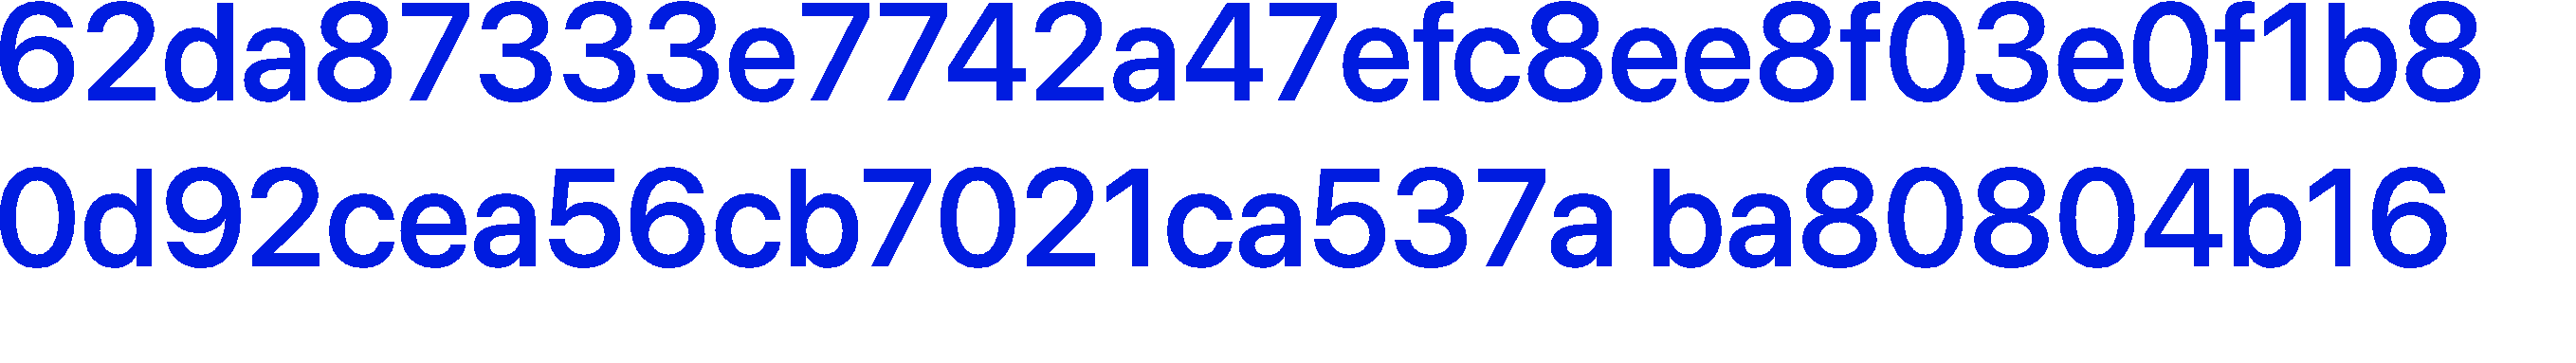
\includegraphics[width=1304\studiounit]{images/studio/collection/figma-0328-part-01.pdf}}
\studiodeclarefield{title}{Hash avalanche}
\studiodeclarefield{text-2}{bOebdc32452d1faa6a20ccf9fOf22d49af\\74f2e0340f4f6981542a56 4b7685c1}
\studiodeclarefield{text-3}{Bitpolito}
\studiodeclarefield{text-4}{BitPolito}
\studioapplyfields
\studiomeasuredcanvas{3556}{2000}{hash-avalanche}{studio-paper}{
\studiomeasuredtext{title}{1351.27}{335.219}{854.992}{170.426}{114.375}{132.675}{\color{bitpolito}\bfseries\centering}{\studiofield{title}}
\studiographfield{graphic-1}{1626}{803}{1304}{184}{}{}
\studiomeasuredtext{text-2}{1625.43}{1265.86}{1309.22}{172.332}{67.9467}{78.8181}{\color{bitpolito}}{\studiofield{text-2}}
\studiomeasuredtext{text-3}{651.582}{818.785}{376.856}{127.101}{84.5507}{98.0788}{\color{bitpolito}}{\studiofield{text-3}}
\studiomeasuredtext{text-4}{651.582}{1280.79}{377.471}{112.634}{84.5467}{98.0741}{\color{bitpolito}}{\studiofield{text-4}}
\path[fill=bitpolito,draw=none,line width=1\studiounit] (1347.5,871)--(1347.5,863.5)--(1185,863.5)--(1185,871)--(1185,878.5)--(1347.5,878.5)--(1347.5,871)--cycle (1415,871)--(1340,827.699)--(1340,914.301)--(1415,871)--cycle;
\path[fill=bitpolito,draw=none,line width=1\studiounit] (1347.5,1333)--(1347.5,1325.5)--(1185,1325.5)--(1185,1333)--(1185,1340.5)--(1347.5,1340.5)--(1347.5,1333)--cycle (1415,1333)--(1340,1289.7)--(1340,1376.3)--(1415,1333)--cycle;
}
